\usetheme{Singapore}
\usepackage{graphicx}
%\usepackage{multimedia}
\logo{
\includegraphics[width = 0.1\textwidth]{hestemlogo}}
\usepackage{keystroke}
\usepackage{marvosym}
\usepackage{ifsym}
%\usepackage{hyperref}
\usepackage{tikz}
\usepackage[tikz]{bclogo}
\usetikzlibrary{arrows,decorations,backgrounds,fit,positioning,calc}
\author{Paul Hewson}
\title{Insights from Data}

\newcommand{\A}{{\color{green}A}}
\newcommand{\B}{{\color{red}B}}
\newcommand{\C}{{\color{blue}C}}
\newcommand{\R}{{\color{red}R}}

\makeatletter
\newcommand{\Repeat}[1]{%
    \expandafter\@Repeat\expandafter{\the\numexpr #1\relax}%
}

\def\@Repeat#1{%
    \ifnum#1>0
        \expandafter\@@Repeat\expandafter{\the\numexpr #1-1\expandafter\relax\expandafter}%
    \else
        \expandafter\@gobble
    \fi
}
\def\@@Repeat#1#2{%
    \@Repeat{#1}{#2}#2%
}
\makeatother


\begin{document}
\mode<article>{\sffamily}

\mode<beamer>{\frame{\titlepage}}

\mode<article>{
\maketitle

\tableofcontents
}






\section{Pre-amble}


\mode<article>{This course has been developed with funding from HE-STEM and in partnership with Devon County Council.   The support of both is gratefully acknowledged.

The aim of the course is to provide a ``one day'' introduction to statistical literacy for use in the workplace.   In doing that, we are trying to make a variety of delivery modes available, a blended course (a combination of online pre-course work, a group contact session and a little online post-course work) as well as a fully online course.   At the time of writing we continue to evaluate the relative merits of each delivery mode.

What this does mean is that for any course, there are online materials, in the form of a Moodle course, which accompanies these notes.   Currently, a live version of these materials are being hosted by the Royal Statistical Society Centre for Statistical Education, and these should allow guest access.   A zip archive of the course is also available for anyone wishing to adopt the course.

All course materials are being offered under the GNU Public Licence.   These learning materials are free to use by anyone, with the sole restriction that you cannot subsequently restrict anyone else's use of these materials.


The course is intended to consist of:
\begin{itemize}
\item Some pre-course activities 
  \begin{itemize}
  \item watch a video, answer some questions about the video
  \item submit ``newspaper'' articles into a database
  \end{itemize}
\item A course - either a ``contact'' session or an entirely online course
\item Some post-course activities
\end{itemize}


}


\mode<article>{\newpage}

\subsection{Activity 1}

\mode<article>{
Following any housekeeping and ice-breaker activities, the course starts with a discussion of the video (and quiz) that was set for pre-reading.
}

\mode<beamer>{

\begin{frame}[label=smidsyvideo]
\frametitle{Pre-course activity 1}

\begin{itemize}
\item You were asked to watch a short video clip, and answer some questions (online).
\item There were few ``correct'' answers, the main point of the exercise was to get you thinking
\item Please now imagine you are a public servant, with finite money to spend on
  \begin{itemize}
  \item An intervention to reduce ``Single vehicle loss of control'' injuries, or
  \item an intervention to reduce ``Sorry Mate I didn't see you collisions''.
  \end{itemize}   
\item In groups, make a decision.   Also, be prepared to explain \emph{why} you chose the intervention you did.
\end{itemize}

\end{frame}

}

\mode<article>{



\includeslide{smidsyvideo}

  \begin{bclogo}[couleur=blue!30, arrondi=0.1, sousTitre=Activity, logo=\bcquestion, ombre=True]{}
Discuss how we priortise an action in this scenario
\end{bclogo}

The fundamental goal of the video exercise was to get people thinking about the evidence we need in order to make a decision about an intervention.  Road travel is a ubiquitous activity.   Many people expect the state (central/local government/police/other) to do ``something'' about road injury.   But how do we decide the priorities.   Part of the discussion could involve the following ideas:

\begin{itemize}
\item Direct resources to what I think is the most important
\item Direct resources to what elected representatives think is most important
\item Direct resources to what the public think is most important
\item Inform a debate on resources using something approaching objective evidence?
\item Balance the needs with the likely effectiveness of any intervention (maybe one problem is more common, but I don't really know how to fix it)
\end{itemize}


Hopefully, we arrive at a position where (a) we see some need for data to support a decision and (b) we acknowledge that these data are unlikely on their own to make the decision for us.  In this case, one major complication may be that some problems are more amenable to our interventions than others.   Even if one crash type were more numerically common than the other, maybe we don't have an effective remedy, and would be better spending our money on something that makes a difference.   However, we should be basing our decisions on data about how common things are, and how effective treatments are.   We shouldn't be basing it on guesswork or anecdote.



}



\frame{
\frametitle{Learning outcome 1}

  \begin{bclogo}[couleur=red!30, arrondi=0.1, sousTitre=GAISE 2010: 1, logo=\bcinfo, ombre=True]{}
Data beat Anecdotes
\end{bclogo}

}


\mode<article>{\newpage}

\subsection{Activity 2}


\mode<beamer>{

\begin{frame}[label=pemdas]
\frametitle{Do we really use data?}

The plural of anecdote IS NOT data

\begin{itemize}
\item<1-> Saying ``data beat anecdotes'' is a cornerstone of statistical literacy
\item<2-> But we contradict it regularly.   
\item<3-> How often do you hear about my dear old Aunt Sally who smokes 80 cigarettes a day, drinks 8 bottles of gin and has still lived to be one hundred and fourteen years old
\item<3-> Who points out that this is ``the exception that proves the rule''
\end{itemize}

\end{frame}

}


\mode<article>{
We first need to address the question of data beating anecdotes.   


\includeslide{pemdas}


With a mature audience, we need to do this in a way that acknowledges the fact that no administrative data (if any data) give a perfect representation of reality.   We therefore have to move to a discussion of decision making in the face of imperfect data.

}

\mode<beamer>{
\begin{frame}[label=jbest]
\frametitle{Joel Best: Lies, Damned Lies and Statistics}

\begin{itemize}
\item Who created this statistic?
\item Why was this statistic created?
\item How was this statistic created?
\end{itemize}

So what?

\begin{itemize}
\item Adopt outright cynicism: don't believe anything based on data ever
\item  Adopt na\"ive acceptance (especially if the ``facts'' suit us).  
\end{itemize}

Both positions have the advantage of being thought free.  However, for a professional, a critically cautious position between these two extremes is needed.

%get that mark twain quote on avoiding thinking

\end{frame}

}


\mode<article>{


\includeslide{jbest}

The aim of of this slide is to prompt a more informed discussion about the actual data that concerns course participants.   What does actually get recorded?   How does it get recorded.   In injury prevention, one ``Gold Standard'' source of data are the police collected, so-called ``STATs 19'' data.

\begin{itemize}
\item Who: collected by the police, in response to information about a collision (so for example, minor collisions involving uninsured drivers may never get reported to the police)
\item Why: apart from the urgent human needs, police involvement is directed towards determining whether an offence has taken place, and whether a prosecution is possible.   This might limit the value of the data for preventative action (if I get hit as a pedestrian / cyclists, I might not care that it was the car driver's fault.   I might care about ways I can prevent it happening again)
\item How: a long, complicated form, sometimes collated in response to a public report a while after the collision occurred.   All evidence is retrospective and ``first impressions''
\end{itemize}

\begin{bclogo}[couleur=blue!30, arrondi=0.1, sousTitre=Activity, logo=\bcquestion, ombre=True]{}
Using other examples provided by the course participants, discuss the limitations of the data using Best's Who/How/Why.
\end{bclogo}

}


\mode<article>{\newpage}

\section{The way we collect data}

\mode<article>{
(Maybe it's time to find a better example).   This case study was used by Sharon Lohr in her excellent (one of the best around) textbook on survey sampling.   There's also an interesting parallel with road injury.   Few people admit to being a ``below average'' driver.   Likewise few people admit to being a ``below average'' lover, so it does seem to have some audience resonance.   We start by stating a few bare ``facts'' from the summary of results.}

\mode<beamer>{
\begin{frame}[label = sherehite]
\frametitle{Shere Hite (1987), Women in Love: A cultural revolution in progress}

\begin{itemize}
\item There were 4,500 respondents to this survey - does that sounds like a big number?   
\item What do you feel is a good number for a survey (note, YouGov predict the election within a few percentage points on smaller numbers than this)
\end{itemize}

\end{frame}
}

\mode<article>{
\includeslide{sherehite}

The aim of this slide is to prompt a discussion about survey methods.   Hopefully, most people would accept that 4,500 is quite large by survey standards.   It is though well worth prompting a discussion about what we mean by ``quite large'', as well as asking about the size of surveys people rely on in their own practice.

  \begin{bclogo}[couleur=blue!30, arrondi=0.1, sousTitre=Activity, logo=\bcquestion, ombre=True]{}
Discuss the validity of results based on a sample size of 4,500.  Discuss the sample sizes used by participants in their own practice.
\end{bclogo}

Once we've exhausted discussion about sample size we can move on to consider the results.}


\mode<beamer>{
\begin{frame}[label=sherehiteresults]
\frametitle{Women in Love?}

\begin{itemize}
\item 84\% of women are not emotionally satisfied with their relationships
\item 70\% of women who have been married for more than 5 years have had affairs
\item 95\% have been emotionally or psychologically harassed by the male
\item 84\% have suffered condescension from the male
\end{itemize}

What is this survey telling us about the wellbeing of women in the US in the 1980s?

\end{frame}
}

\mode<article>{

\includeslide{sherehiteresults}

This should fuel a good open ended discussion.   The findings out to be a little challenging.   It is worth letting this discussion run, with careful prompting.   I suppose it's bad pedagogy to let anyone comprehensively challenge a theory of human relationships before you display the next slide, but the more people try to engage with the results the better

  \begin{bclogo}[couleur=blue!30, arrondi=0.1, sousTitre=Activity, logo=\bcquestion, ombre=True]{}
Discuss the findings of Shere Hite's survey.
\end{bclogo}

}  

\mode<beamer>{

\begin{frame}[label=sherehiteresponse]
\frametitle{Women who fill in surveys in Love}

\begin{itemize}
\item 100,000 surveys were sent out, only 4,500 came back
\item There were 127 essay type questions
\item Are the 4,500 women who filled in such a survey typical of the 100,000 who were invited to take part?   Are the 100,000 who were invited to take part typical of women in the US in the 1980s
\end{itemize}

\end{frame}
}

\mode<article>{

\includeslide{sherehiteresponse}

It is this last slide on response rate that really provides the key to the results presented.   It is worth giving more information on the way the data were collected.   Actually 100,000 surveys were sent out, only 4,500 came back.   It may well be that those 100,000 surveys were sent to an essentially representative sample frame (alhough that is a little unlikely).   But the key point is that we have a 4.5\% response rate.   In addition, there were 127 essay type questions.   So the concluding question we leave with is ``will the 4.5\% of respondents (who are willing to write all those essays about intimate aspects of their life) be typical of US women?''

  \begin{bclogo}[couleur=blue!30, arrondi=0.1, sousTitre=Activity, logo=\bcquestion, ombre=True]{}
Discuss the validity of the conclusions in the light of the low response rate
\end{bclogo}

Hopefully at this point the audience will be ready to discuss the next point.

}

\frame{
\frametitle{Learning outcome 2}

  \begin{bclogo}[couleur=red!30, arrondi=0.1, sousTitre=GAISE 2010: 2, logo=\bctakecare, ombre=True]{}
Random sampling allows results of surveys %and experiments 
to be extended to the
population from which the sample was taken.
%Random sampling from a population is what allows us to understand the population to which they apply.
\end{bclogo}

}




\mode<beamer>{

\begin{frame}[label=surveydiscussion]
\frametitle{Surveys or data?}
\begin{itemize}
\item There are large national surveys (carried out by agencies or national statistical bodies) which use fairly sophisticated variations on ``random sampling'', but done in a way they can produce results that are ``representative'' (think about election forecasting).
\item What about the surveys we commission locally / use locally?   
\item What problems might there be with non-response?
\item Do we think these are representative?
\item What could we do to make them more representative?
\end{itemize}


\end{frame}

\begin{frame}[label=whatpop]
\frametitle{What's the population}

\begin{itemize}
\item A big part of understanding (and designing) surveys is thinking about the relevant population
\end{itemize}
\end{frame}

}

\mode<article>{


\includeslide{surveydiscussion}

First, we need to make a technical point (about non-response) and the value of random sampling.   It can be a strange idea to think that randomly selected people can ``represent'' a population.

But secondly, we need to think carefully about the ``population to which these results apply''

\includeslide{whatpop}


  \begin{bclogo}[couleur=blue!30, arrondi=0.1, sousTitre=Activity, logo=\bcquestion, ombre=True]{}
Discuss the target ``population'' which is being examined by this survey.   Consider examples provided by the course participants.
\end{bclogo}

}



\mode<beamer>{
\begin{frame}[label=brakemobilephone]
\frametitle{Mobile Phone Killer Crash Risk}

Source: www.brake.org.uk/handheld-mobile-phone-use-one-rise-brake-reaction

\begin{itemize}
\item Survey of 21 year old students
\item Is that typical
\end{itemize}
\end{frame}
}

\mode<article>{
\includeslide{brakemobilephone}

The slide above is typical of one that has been submitted by a course participant in the pre-course activities.   The aim now is to discuss carefully what this headline is telling us

}





\mode<beamer>{

\frame{
  \frametitle{Happiness Census}

100 people questioned, all respond.

%\Smiley

%\Repeat{0}{test }

\Large
\Repeat{20}{{\color{red}\Smiley }}

\Repeat{20}{{\color{red}\Smiley }}

\Repeat{20}{{\color{red} \Smiley }} 

\Repeat{20}{{\color{red} \Smiley }} 

\Repeat{20}{{\color{blue} \Frowny }}

%\Repeat{3}{test }

%\Repeat{4}{test }

%\Repeat{5}{test }

\normalsize

\begin{itemize}
\item 80 / 100 are happy, the proportion of happy people is 80\%
\item If this were a random sample of (say) 1,000 students we could do something ``statistical'' (compute a confidence interval for the proportion of happy students in the population).  But we don't need to.    Here, 100 is the population
\end{itemize}

}


\frame{
  \frametitle{Happiness Census}

More realistically, 100 people questioned, 60 respond.

%\Smiley

%\Repeat{0}{test }

\Large
\Repeat{20}{{\color{red}\Smiley}}

\Repeat{20}{{\color{red}\Smiley}} 

\Repeat{8}{{\color{red}\Smiley}}\Repeat{12}{{\color{blue}\Frowny}}

\normalsize
\Repeat{20}{{\color{gray}\Neutral}} 

\Repeat{20}{{\color{gray}\Neutral}}

%\Repeat{3}{test }

%\Repeat{4}{test }

%\Repeat{5}{test }


\normalsize

\begin{itemize}
\item 48 / 60 are happy; the proportion of happy people \emph{\color{red}who responded to the ``survey''} is 80\%
\item We \emph{\color{blue}can}\footnote{\color{blue}although we shouldn't} plug these numbers into a computer and do something statistical to get a 95\% confidence interval for the \emph{\color{red}population} proportion as (68\%, 88\%).   But just see how silly that is on the next two slides.
\end{itemize}

}






\frame{
  \frametitle{If all the non-responders were too busy being happy to sit behind a computer filling in surveys}

100 people questioned, 60 respond.

%\Smiley

%\Repeat{0}{test }

\Large
\Repeat{20}{{\color{red}\Smiley}}

\Repeat{20}{{\color{red}\Smiley}} 

\Repeat{8}{{\color{red}\Smiley}}\Repeat{12}{{\color{blue}\Frowny}}

\Repeat{20}{{\color{gray}\Smiley}} 

\Repeat{20}{{\color{gray}\Smiley}}

%\Repeat{3}{test }

%\Repeat{4}{test }

%\Repeat{5}{test }

\normalsize

\begin{itemize}
\item In the population, we have 88 / 100 who are are happy; the proportion of happy people \emph{\color{red}in the population} is 88\%
\end{itemize}
}




\frame{
  \frametitle{Or if all the non-responders were too fed up to fill in surveys (no computers, we didn't teach them how to use computers etc.)}

100 people questioned, 60 respond.

%\Smiley

%\Repeat{0}{test }

\Large
\Repeat{20}{{\color{red}\Smiley}}

\Repeat{20}{{\color{red}\Smiley}} 

\Repeat{8}{{\color{red}\Smiley}}\Repeat{12}{{\color{blue}\Frowny}}

\Repeat{20}{{\color{gray}\Frowny}} 

\Repeat{20}{{\color{gray}\Frowny}}


\normalsize

\begin{itemize}
\item In the population, we have 48 / 100 who are are happy; the proportion of happy people \emph{\color{red}in the population} is 48\%
\end{itemize}
}


\frame{
\frametitle{Non-response to surveys}

\begin{itemize}
\item Non-response is a real problem
\item There are some (really quite advanced, i.e., rather specialised, i.e., think expensive expert) methods which try to help out.   Clever as they are (i.e., I like playing with them) they are not a magic wand.
\item Putting effort into minimising non-response (or at least understanding who is and isn't responding) is really quite important
\end{itemize}

}

}

\mode<article>{\newpage}

\section{Randomness is Natural}


\mode<article>{
I've just bought myself a full size Alan Sugar facemask to make this next exercise a little more interesting.   However, the basic idea is one of W.Edwards Deming.


\begin{itemize}
\item Get (about) 8 volunteers
\item Give them a task.   I have used sampling beads from an urn (``make batches of yellow beads'', I have used die (``get a five or a six'') and I have used coins (``throw the coin eight times and get at least six heads'').
\item Collect results from the volunteers.   Put on the Alan Sugar mask and ``fire'' the worst performing individual.   Promote the best performing individual (who is now called Karen or Nick).   Maybe put a big ``D'' hat on anyone who almost got fired.   Run another round.
\item Fire/promote/reward as necessary
\item Repeat until there is a winner, who gets a bag of chocolates or other token prize
\end{itemize}

At this point we can have an interesting discussion about ``fairness''.   One advantage of the dice/coins is that we can fairly easily get a sense of what a typical value should be.   In fact, we can even formalise this as an expected value.

  \begin{bclogo}[couleur=blue!30, arrondi=0.1, sousTitre=Activity, logo=\bcquestion, ombre=True]{}
Carry out this (Deming) based illustration of randomness.   Discuss the fairness of the findings.   Consider expected value if appropriate.
\end{bclogo}

 
}


\mode<beamer>{

\begin{frame}[label=pi1]
\frametitle{Fictional performance indicator}

\includegraphics[width=0.7\textwidth]{pi1}

\end{frame}

\begin{frame}[label=pi2]
\frametitle{How we normally use these data}

\includegraphics[width=0.7\textwidth]{pi2}

\end{frame}


\begin{frame}[label=pi3]
\frametitle{Isn't this just random blips either side of a trend?}

\includegraphics[width=0.7\textwidth]{pi3}

\end{frame}

}

\mode<article>{
We close this session with some fictional (or some real, if it's available) Performance INdicator data.  

\includeslide{pi1}

This kind of slide is familiar (maybe we don't even need the trend to start with)

\includeslide{pi2}

And this kind of treatment is familiar.


\includeslide{pi3}

So the final slide should prompt a bit of a discussion.   How do we determine trends (and should they be rewarded for the trend?); how do we determine blips.   I've often ended up explaining things like CUSUM charts at this point - maybe something should be added.    We want to avoid cynicism (it's all randomness).   But most of the course participants I've had to date are the subject of performance monitoring and perhaps would expect the producers to give them the information as a CUSUM chart.

  \begin{bclogo}[couleur=blue!30, arrondi=0.1, sousTitre=Activity, logo=\bcquestion, ombre=True]{}
Discuss the importance of distinguishing signal from noise (randomness from substantive)
\end{bclogo}

}



\mode<beamer>{
\begin{frame}[label=allmakeheads]
\frametitle{Modelling randomness}

\begin{itemize}
\item Now we need everyone to toss a coin six times
\item Count the number of heads
\item (we may need to do this a second time if the numbers are small)
\item Let's graph the results
\end{itemize}

\end{frame}


\begin{frame}[label=binomial]
\frametitle{One theoretical model}

\begin{displaymath}
P[X=x] = \binom{n}{x} p^x (1-p)^{n-x}
\end{displaymath}

\begin{center}
\includegraphics[width = 0.5\textwidth]{binom}
\end{center}

\end{frame}


}

\mode<article>{
We can do a simple experiment to try to persuade people we have models for randomness.   Get everyone to toss six coins, and record the number of heads they get (if it's a very small group they may have to do this twice).

\includeslide{allmakeheads}

We can collate the results as a bar/tally graph, and compare them with a simple theoretical model (the binomial)

\begin{tabular}{l|l}
Heads & People \\
\hline
0 &  \\
1 & $\times$ %\StrokeOne
 \\
2 & $\times \times \times$%\StrokeThree
 \\
3 & $\times \times \times \times \times \times \times $%\StrokeFive \StrokeThree
\\
4 & $\times  \times $ %\StrokeTwo
 \\
5 &  \\
6 & $\times$ %\StrokeOne
 \\
\end{tabular}

We can compare this flipchart/whiteboard with the theoretical model below


  \begin{bclogo}[couleur=blue!30, arrondi=0.1, sousTitre=Activity, logo=\bcquestion, ombre=True]{}
Get everyone to carry out a coin tossing experiment.   Collate the results.   Compare them to the ``theoretical'' model.
\end{bclogo}

\includeslide{binomial}

}

\frame{
\frametitle{Learning outcome 3}

  \begin{bclogo}[couleur=red!30, arrondi=0.1, sousTitre=GAISE 2012: 2, logo=\bctakecare, ombre=True]{}
Variability is natural and is also predictable and quantifiable
\end{bclogo}


}




\mode<article>{\newpage}



\section{Contextual variables}

\mode<article>{

We are going to ``drift'' towards causation (it's such a difficult subject).   Again, it helps partipants reflect on their own practice to think about contextual variables that are relevant to them. 


Your task is to consider all the things you could potentially measure which might have a bearing on your practice.   In a road safety context for example we might consider weather, vehicle safety, highway design, training programmes.  
}


\mode<beamer>{
\begin{frame}[label=contextual]
\frametitle{Contextual variables}

What affects the success of your practice.   Consider both:

\begin{itemize}
\item Intrinsic factors
\item Extrinsic factors
\end{itemize}

(This slide isn't intended to add to jargon overload - it's to highlight the fact you should think of things you control as well as things that are beyond your control)

\end{frame}

}



\mode<article>{

\includeslide{contextual}


  \begin{bclogo}[couleur=blue!30, arrondi=0.1, sousTitre=Activity, logo=\bcquestion, ombre=True]{}
Collate lists of relevant contextual variables for the participants practice
\end{bclogo}

To make this illustration a little concrete, here are a number of possibilities for road injury prevention.



\frame{
\frametitle{For road injury prevention}

\begin{itemize}
\item Newspaper articles
\item Accident signs (requests for witnesses, ``hotspots'')
\item Insurance
\item 999 calls
\item STATs19, Ambulance, F\&R, HES, A\&E
\item Other
\end{itemize}


}

\frame{
\frametitle{Contextual variables}

\begin{itemize}
\item New / existing driving licences
\item New / existing cars; car tax, MOTs
\item Trafic surveys
\item Perception surveys
\item Demographics
\item Car tax
\item Census
\item Car manufacturer surveys
\item Many more
\end{itemize}

}


We had quite an interesting time teasing this out (for example newspapers might report insurance figures, so what's data and what's not).



\subsection{Lurking variables}

As part of our drift towards causation, we wanted to talk about lurking variables. 

}

\mode<beamer>{

\begin{frame}[label=lurking]
\frametitle{Illustrating Lurking variables}

\begin{itemize}
\item There is a correlation between weekly gas sales and weekly deaths of old people (in the UK).   Why?
%\item<2-> Probably because of the weather.   
\end{itemize}

% \begin{tikzpicture}[node distance = 5mm,
%   nonterminal/.style={
%   rectangle,minimum size=6mm,very thick,draw=red!50!black,top
%   color=white,text width = 2.5cm,text centered},
% terminal/.style={
%   rectangle,rounded corners=3mm,minimum size=6mm,text width = 2cm,text centered,very thick,draw=red!20!black,top
%   color=white}
% ]
% %\usetikzlibrary{fit}
% %\usetikzlibrary{calc}
% % ...

% \node(L)[nonterminal]{ Weather};
% \node(B)[terminal,right=of L]{Gas sales};
% \node(C)[terminal,below=of B]{Elderly Deaths};
% \
% \draw[->] (L) -- (B); 

% \draw[->] (L) -- (C); 

% \draw[->] (C) -- (B); 

% %\draw[red,ultra thick,rounded corners] (7.5,5.3) rectangle (9.4,6.2);
% %\node(E)[terminal,below=of D]{Stop};

% %\node [draw,circle] (A) {Text};
% %\node [draw,fit=(A) (A.west - 3cm)] {};

% \end{tikzpicture}
\end{frame}




\begin{frame}[label=elderlydeath]
\frametitle{Lurking variables}

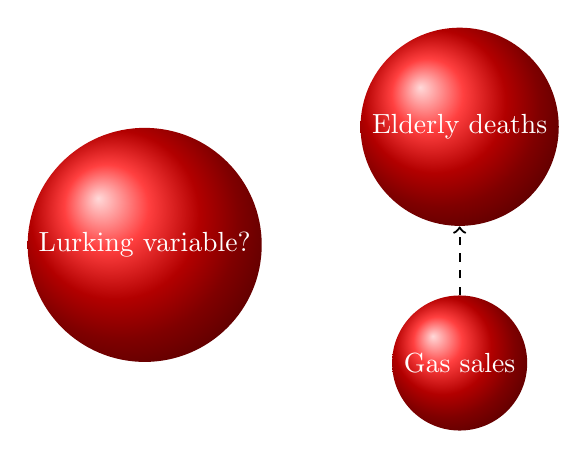
\begin{tikzpicture}
[parent anchor = east,child anchor = west, grow = east,
every  node/.style={ball color=red,circle,text=white},
edge from parent/.style={draw,dashed,thick,red}]
\node{Lurking variable?}
[level distance=40mm, sibling distance = 30mm]
  child {node (a) {Gas sales} edge from parent[draw=none]}
  child {node (b) {Elderly deaths} edge from parent[draw=none]};
\draw[dashed,->,thick] (a) -- (b);
\end{tikzpicture}

\end{frame}


\begin{frame}[label=elderlydeathexplained]
\frametitle{Weather as a lurking variable}

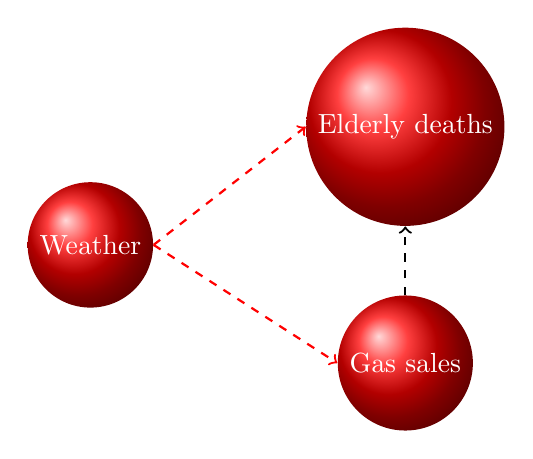
\begin{tikzpicture}
[parent anchor = east,child anchor = west, grow = east,
every  node/.style={ball color=red,circle,text=white},
edge from parent/.style={draw,dashed,thick,red}]
\node{Weather}
[level distance=40mm, sibling distance = 30mm]
  child {node (a) {Gas sales} edge from parent[dashed,->]}
  child {node (b) {Elderly deaths} edge from parent[dashed,->]};
\draw[dashed,->,thick] (a) -- (b);
\end{tikzpicture}

\end{frame}



\begin{frame}[label=elderlydeathsummary]
\frametitle{In other words}

\begin{itemize}
\item There is an apparent association between gas sales and elderly deaths
\item But the reason for this association is probably due to weather.   Weather is associated with both the elderly death \emph{and} the gas sale variable
\end{itemize}

This is a key idea, and worth careful discussion.   We shall review several of the news items that have been submitted and see where we need to think about lurking variables.


\end{frame}


}


\mode<article>{

We now run through a series of visuals which illustrate the idea of a lurking variable (epidemiologists call this a confounding variable - I prefer ``lurking'' as it's less jargon sounding).

\includeslide{lurking}

We set up one slide to explain the general idea.


\includeslide{elderlydeath}

Then we illustrate it with a rather famous (if overused) example.

\includeslide{elderlydeathexplained}

And then explain the idea of ``lurking'' variable.

\includeslide{elderlydeathsummary}


Finally, we summarise the basic idea.



The next step is to consolidate this, using examples that have been submitted by the course participants.

}

\frame{
\frametitle{Exhibit 1: ``Male road accidents soar in summer due to women's short skirts''}

\begin{quote}
``The scorching heatwave in early July caused road accidents to soar because male drivers were distracted by womens' skimpy outfits, according to insurance claim figures.''
\end{quote}

Source: Telegraph Online Posted 7:00am BST 30th Jul 2010
http://www.telegraph.co.uk/motoring/news/7917861/Male-road-accidents-soar-in-summer-due-to-womens-short-skirts.html

\begin{quotation}
``And according to car insurance company Sheilas' Wheels, the summer smash phenomenon is getting worse each year - in 2009 men made 16.4 per cent more claims during the Summer than in any other month.''
\end{quotation}


}



\frame{
\frametitle{Lurking variables}

Suggest possible lurking variables:

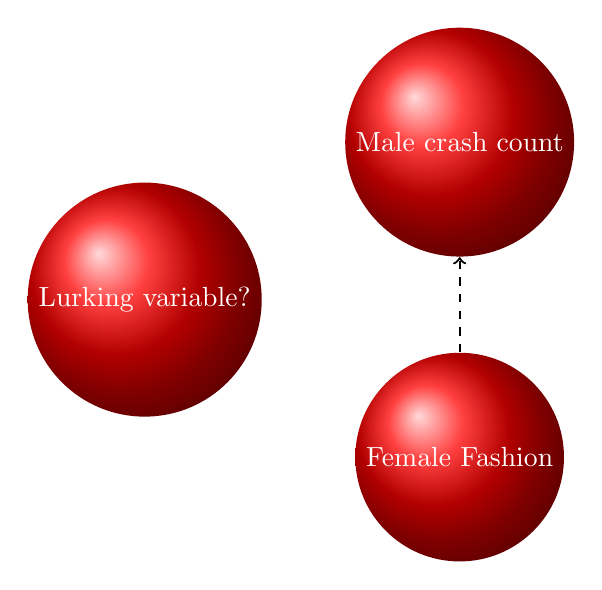
\begin{tikzpicture}
[parent anchor = east,child anchor = west, grow = east,
every  node/.style={ball color=red,circle,text=white},
edge from parent/.style={draw,dashed,thick,red}]
\node{Lurking variable?}
[level distance=40mm, sibling distance = 40mm]
  child {node (a) {Female Fashion} edge from parent[draw=none]}
  child {node (b) {Male crash count} edge from parent[draw=none]};
\draw[dashed,->,thick] (a) -- (b);
\end{tikzpicture}

}


\mode<article>{

  \begin{bclogo}[couleur=blue!30, arrondi=0.1, sousTitre=Activity, logo=\bcquestion, ombre=True]{}
Using material provided by the participants, consider possible lurking variables for any apparent associations seen.
\end{bclogo}


For the Sheila's wheel example, we came up with many possible lurking variables (essential all to do with summer, e.g. in summer you get dazzled, you travel to the beach and so on).   Another example could be Speed and Accident rate.   A lurking variable could be ``Young drivers'' (who have various bad practices including dangerous overtaking and tailgating)


}


\mode<article>{\newpage}


\section{Experiments}

\mode<beamer>{

\begin{frame}[label=causation]
\frametitle{A word on causation}

\begin{enumerate}
\item Sometimes we collect data to prioritise, to explore a phenomenon
\item Sometimes we collect data in order to understand whether certain attributes (behaviours/people) are more likely to lead to worse outcomes
\item Sometimes we collect data as part of a study in order to decide whether an intervention ``works''
\end{enumerate}

Motive 1 is all about exploration.   Motives 2 and 3 are about causation.   However, for ethical reasons, we can usually only get really strong evidence of causation for Motive 3.


\end{frame}

}

\mode<article>{
I'm almost frightened of using the phrase ``causation'', but we have to cover the topic.  

\includeslide{causation}

In my (biased and limited) experience, I'm usually dealing with people who have observational data (and quite often it's secondary observational data).   They also want to understand causation.   And, as Oscar Wilde said, (approximiately) sometimes you have to pay attention to circumstantial evidence, such as when you find a fish in your milk.     So saying that observational studies tell us nothing about causation is going to be very challenging idea indeed.   It also might suit some people to be able to dismiss any and all observational studies they don't like, and revert to their common sense as a guide to causation.

So I think we need to travel this topic carefully.

There are two sets of materials.   One is that I run an experiment,  based on an idea passed on to me by Mark Kent of (now) Solihull College.   This needs to be timed carefully.

}

\mode<beamer>{
\begin{frame}[label=markkent]
\frametitle{A simple memory test}

An experiment to determine whether sugar in chocolate enhances performance in a memory test.

\begin{itemize}
\item Put all your pens down.
\item You will be read a sequence of 8 numbers.
\item You may then pick up your pens, and write down the sequence from memory.
\item We will then mark how many you got right.   Maximum mark is 8, but to get a mark the number must be in exactly the right position (so if you get four right, miss one altogether, and get the next three right you only get four marks as the last three will be out of position)
\item When we've done this once, I will tell you to eat the chocolate.
\item After 12 minutes, we will repeat the exercise
\end{itemize}

\end{frame}


}


\mode<article>{
\includeslide{markkent}


Possibly this is bad practice.  I run this chocolate experiment with numbers such as these:

\begin{itemize}
\item[Before] 3,1,5,4,3,8,5,6
\item[After]  8,2,5,2,6,4,5,9
\end{itemize}

Generally (but not always) we get better performance second time around.   The aim of the exercise is to discuss whether we think we've proved the idea that the sugar in chocolate improves performance in a memory test.

Usually, the discussion converges around the idea that there is a training effect (second time round the students know what on earth was going on).   It is possible to use diabetic chocolate to entirely rule out the idea that sugar had anything to do with it.   I also forgot the chocolate once and had to use water with a story about brain hydration.   You usually get some very good suggestions (at a Masterclass, a year 9 pupil told me they did better because I had told them they would do better).   But essentially, this little demonstration usually gets us to the idea that we needed a control group (and maybe they should have a placebo of sugar free/caffeine free chocolate).

  \begin{bclogo}[couleur=blue!30, arrondi=0.1, sousTitre=Activity, logo=\bcquestion, ombre=True]{}
Carry out the memory test/chocolate eating experiment.
\end{bclogo}

Partly as a time filler, partly as an explanation of \emph{why} randomisation works, I run through the following slides while we are waiting for the 12minutes to expire.

}

 
\mode<beamer>{

\begin{frame}[label=simpson1]
  \frametitle{Flu remedy}

Consider the following fictitious data:

\begin{center}
\begin{tabular}{|l|r|r|r|r|}
\hline
&  Pain &  No pain  & Total  &  Percent with\\
Treatment & relief & relief & number & pain relief \\
\hline
Remedy & 386 & 414 & 800 & {\color{red}48\%} \\
Control & 317 & 483 & 800 & {\color{red}40\%}\\
\hline
Total & 703 & 897 & 1,600 & \\
\hline
\end{tabular}
\end{center}

\begin{itemize}
\item It is summarised as A $2 \times 2$ contingency table
\item Your question: is the ``Remedy'' better than the control
\end{itemize}

\end{frame}


\begin{frame}[label=simpson2]
  \frametitle{Females}

Now consider a subgroup analysis of half the study group.

\begin{center}
\begin{tabular}{|l|r|r|r|r|}
\hline
&  Pain &  No pain  & Total  &  Percent with\\
Treatment & relief & relief & number & pain relief \\
\hline
Remedy  &  351 & 249 & 600 & {\color{red}59\%}\\
Control & 142 &  58 &  200 & {\color{red}71\%}\\
\hline
\end{tabular}
\end{center}


\begin{itemize}
\item Your question: does the remedy ``work'' for this subgroup
\end{itemize}

\end{frame}

\begin{frame}[label=simpson3]
  \frametitle{Males}

And just to be fair, let's consider the other subgroup

\begin{center}
\begin{tabular}{|l|r|r|r|r|}
\hline
&  Pain &  No pain  & Total  &  Percent with\\
Treatment & relief & relief & number & pain relief \\
\hline
Remedy &    35 &  165  & 200 & {\color{red}18\%}\\
Control & 175  & 425 & 600 & {\color{red}30\%}\\
\hline
\end{tabular}
\end{center}

\begin{itemize}
\item Your question: does the remedy work for this subgroup?
\end{itemize}

\end{frame}


\begin{frame}[label=simpson4]
\frametitle{What's going on}

\begin{itemize}
\item<1-> I think the top level table implies that the remedy ``works''.   48\% of people taking the remedy had pain relief, which is better than the 40\% who took the control
\item<2-> Clearly, plenty of people who took the control had pain relief.  
\item<3-> But in some sense, you seem to increase your chance of pain relief if you take the remedy
\item<4-> Provided there are no worrysome costs (cash or side effect wise) incurred by taking the remedy it seems better to take the remedy
\end{itemize}

\end{frame}


\begin{frame}[label=simpson5]
\frametitle{The paradox}

\begin{itemize}
\item More females (600) than males (200) took the remedy
\item Whatever treatment they take, females are more likely (59\%, 71\%) to report pain relief than males (18\%, 30\%)
\item Combine the two points, and we have a situation where the top level results completely contradict the subgroup results
\item Although these are fictitious data, we can find plenty of real world examples
\end{itemize}

\end{frame}


\begin{frame}[label=simpson6]
\frametitle{Random allocation}

\begin{itemize}
\item Had we randomly allocated subjects to remedy or control, we would have (roughly) as many males and females in each group.   
\item We could ``randomise away'' the systematic differences between males and females.
\item Now, if we have all kinds of other systematic differences (long sighted people / short sighted people, quick reaction time/slow reaction time), we couldn't identify all the possible subgroups.
\item However, hopefully the random allocation process spreads these systematic differences out evenly
\item So hopefully, the only systematic difference between the two groups is that they received a different experimental treatment
\item And we therefore hope that any differences we observe between the two groups can be attributed to that treatment.
\end{itemize}

\end{frame}

}

\mode<article>{

Without getting into the jargon (i.e. never mentioning Simpson's / Yule's paradox) we run through a few slides which demonstrate (again) another lurking variable problem.

\includeslide{simpson1}

The first slide should also allow room for discussion on what we mean by a good treatment effect.

\includeslide{simpson2}

The second slide is a good place to ask people what is going to happen when we show the next slide.   A few smarties guess that we are playing tricks on them, but provided we focus on reasoning people should be clear that if headline figures go one way, and females go another, then males should very strongly match the headline direction.

\includeslide{simpson3}

It can be good to run through some of the arithmetic just to verify what's going on.


\includeslide{simpson4}

Nowadays, following advice given in a causeweb seminar, I never mention the name of this paradox (too much jargon).   I also try to get the group to work out how this has happened before I give the answer away (nearly always someone spots that males and females have taken different numbers of remedy / control).   Rarely someone makes the full link (that females recover better from flu than males).

I then try to conclude the chocolate experiment before moving on.   The next two slides summarise everything here.

\includeslide{simpson5}

\includeslide{simpson6}

}



\frame{
\frametitle{Learning Outcome}


  \begin{bclogo}[couleur=red!30, arrondi=0.1, sousTitre=GAISE 2010: 4, logo=\bcinfo, ombre=True]{}
Random assignment in comparative experiments allows cause and effect
conclusions to be drawn.
%Random allocation is what allows us to determine cause and effect
\end{bclogo}

\begin{itemize}
\item The fundamental contribution of statistics to experiments is in terms
of \emph{randomisation}.   
\item This is a most powerful way of dealing with
potential confounding variables.   Not only do we reduce the risk of
confounding (by averaging it out across all experimental groups) but
we can actually measure the remaining uncertainty.
\end{itemize}

}



\mode<article>{


The conclusion here is that in some circumstances, there ought to be data from controlled experiments on the effectiveness of interventions.   Perhaps such studies should guide our practice, rather than our own tinkerings.

However, determining causality in order to understand why (bad) things happen is a little more complex, and may require futher discussion.







%\includeslide{slide1}


}

\frame{
\frametitle{Post course work}

\begin{itemize}
\item 
\item Motorcycle crashes and ownership over time.
\item Darrel Huff - some misleading visuals
\end{itemize}

}




\end{document}